\documentclass[twoside]{book}

% Packages required by doxygen
\usepackage{fixltx2e}
\usepackage{calc}
\usepackage{doxygen}
\usepackage[export]{adjustbox} % also loads graphicx
\usepackage{graphicx}
\usepackage[utf8]{inputenc}
\usepackage{makeidx}
\usepackage{multicol}
\usepackage{multirow}
\PassOptionsToPackage{warn}{textcomp}
\usepackage{textcomp}
\usepackage[nointegrals]{wasysym}
\usepackage[table]{xcolor}

% Font selection
\usepackage[T1]{fontenc}
\usepackage[scaled=.90]{helvet}
\usepackage{courier}
\usepackage{amssymb}
\usepackage{sectsty}
\renewcommand{\familydefault}{\sfdefault}
\allsectionsfont{%
  \fontseries{bc}\selectfont%
  \color{darkgray}%
}
\renewcommand{\DoxyLabelFont}{%
  \fontseries{bc}\selectfont%
  \color{darkgray}%
}
\newcommand{\+}{\discretionary{\mbox{\scriptsize$\hookleftarrow$}}{}{}}

% Page & text layout
\usepackage{geometry}
\geometry{%
  a4paper,%
  top=2.5cm,%
  bottom=2.5cm,%
  left=2.5cm,%
  right=2.5cm%
}
\tolerance=750
\hfuzz=15pt
\hbadness=750
\setlength{\emergencystretch}{15pt}
\setlength{\parindent}{0cm}
\setlength{\parskip}{3ex plus 2ex minus 2ex}
\makeatletter
\renewcommand{\paragraph}{%
  \@startsection{paragraph}{4}{0ex}{-1.0ex}{1.0ex}{%
    \normalfont\normalsize\bfseries\SS@parafont%
  }%
}
\renewcommand{\subparagraph}{%
  \@startsection{subparagraph}{5}{0ex}{-1.0ex}{1.0ex}{%
    \normalfont\normalsize\bfseries\SS@subparafont%
  }%
}
\makeatother

% Headers & footers
\usepackage{fancyhdr}
\pagestyle{fancyplain}
\fancyhead[LE]{\fancyplain{}{\bfseries\thepage}}
\fancyhead[CE]{\fancyplain{}{}}
\fancyhead[RE]{\fancyplain{}{\bfseries\leftmark}}
\fancyhead[LO]{\fancyplain{}{\bfseries\rightmark}}
\fancyhead[CO]{\fancyplain{}{}}
\fancyhead[RO]{\fancyplain{}{\bfseries\thepage}}
\fancyfoot[LE]{\fancyplain{}{}}
\fancyfoot[CE]{\fancyplain{}{}}
\fancyfoot[RE]{\fancyplain{}{\bfseries\scriptsize Generated by Doxygen }}
\fancyfoot[LO]{\fancyplain{}{\bfseries\scriptsize Generated by Doxygen }}
\fancyfoot[CO]{\fancyplain{}{}}
\fancyfoot[RO]{\fancyplain{}{}}
\renewcommand{\footrulewidth}{0.4pt}
\renewcommand{\chaptermark}[1]{%
  \markboth{#1}{}%
}
\renewcommand{\sectionmark}[1]{%
  \markright{\thesection\ #1}%
}

% Indices & bibliography
\usepackage{natbib}
\usepackage[titles]{tocloft}
\setcounter{tocdepth}{3}
\setcounter{secnumdepth}{5}
\makeindex

% Hyperlinks (required, but should be loaded last)
\usepackage{ifpdf}
\ifpdf
  \usepackage[pdftex,pagebackref=true]{hyperref}
\else
  \usepackage[ps2pdf,pagebackref=true]{hyperref}
\fi
\hypersetup{%
  colorlinks=true,%
  linkcolor=blue,%
  citecolor=blue,%
  unicode%
}

% Custom commands
\newcommand{\clearemptydoublepage}{%
  \newpage{\pagestyle{empty}\cleardoublepage}%
}

\usepackage{caption}
\captionsetup{labelsep=space,justification=centering,font={bf},singlelinecheck=off,skip=4pt,position=top}

%===== C O N T E N T S =====

\begin{document}

% Titlepage & ToC
\hypersetup{pageanchor=false,
             bookmarksnumbered=true,
             pdfencoding=unicode
            }
\pagenumbering{alph}
\begin{titlepage}
\vspace*{7cm}
\begin{center}%
{\Large My Project }\\
\vspace*{1cm}
{\large Generated by Doxygen 1.8.13}\\
\end{center}
\end{titlepage}
\clearemptydoublepage
\pagenumbering{roman}
\tableofcontents
\clearemptydoublepage
\pagenumbering{arabic}
\hypersetup{pageanchor=true}

%--- Begin generated contents ---
\chapter{Hierarchical Index}
\section{Class Hierarchy}
This inheritance list is sorted roughly, but not completely, alphabetically\+:\begin{DoxyCompactList}
\item \contentsline{section}{Board}{\pageref{class_board}}{}
\begin{DoxyCompactList}
\item \contentsline{section}{Property}{\pageref{class_property}}{}
\begin{DoxyCompactList}
\item \contentsline{section}{Railroad}{\pageref{class_railroad}}{}
\end{DoxyCompactList}
\end{DoxyCompactList}
\item \contentsline{section}{Chnc\+Com}{\pageref{class_chnc_com}}{}
\item \contentsline{section}{Die}{\pageref{class_die}}{}
\item \contentsline{section}{Player}{\pageref{class_player}}{}
\item \contentsline{section}{Rules}{\pageref{class_rules}}{}
\end{DoxyCompactList}

\chapter{Class Index}
\section{Class List}
Here are the classes, structs, unions and interfaces with brief descriptions\+:\begin{DoxyCompactList}
\item\contentsline{section}{\hyperlink{class_board}{Board} }{\pageref{class_board}}{}
\item\contentsline{section}{\hyperlink{class_chnc_com}{Chnc\+Com} }{\pageref{class_chnc_com}}{}
\item\contentsline{section}{\hyperlink{class_die}{Die} }{\pageref{class_die}}{}
\item\contentsline{section}{\hyperlink{class_player}{Player} }{\pageref{class_player}}{}
\item\contentsline{section}{\hyperlink{class_property}{Property} }{\pageref{class_property}}{}
\item\contentsline{section}{\hyperlink{class_railroad}{Railroad} }{\pageref{class_railroad}}{}
\item\contentsline{section}{\hyperlink{class_rules}{Rules} }{\pageref{class_rules}}{}
\end{DoxyCompactList}

\chapter{Class Documentation}
\hypertarget{class_board}{}\section{Board Class Reference}
\label{class_board}\index{Board@{Board}}
Inheritance diagram for Board\+:\begin{figure}[H]
\begin{center}
\leavevmode
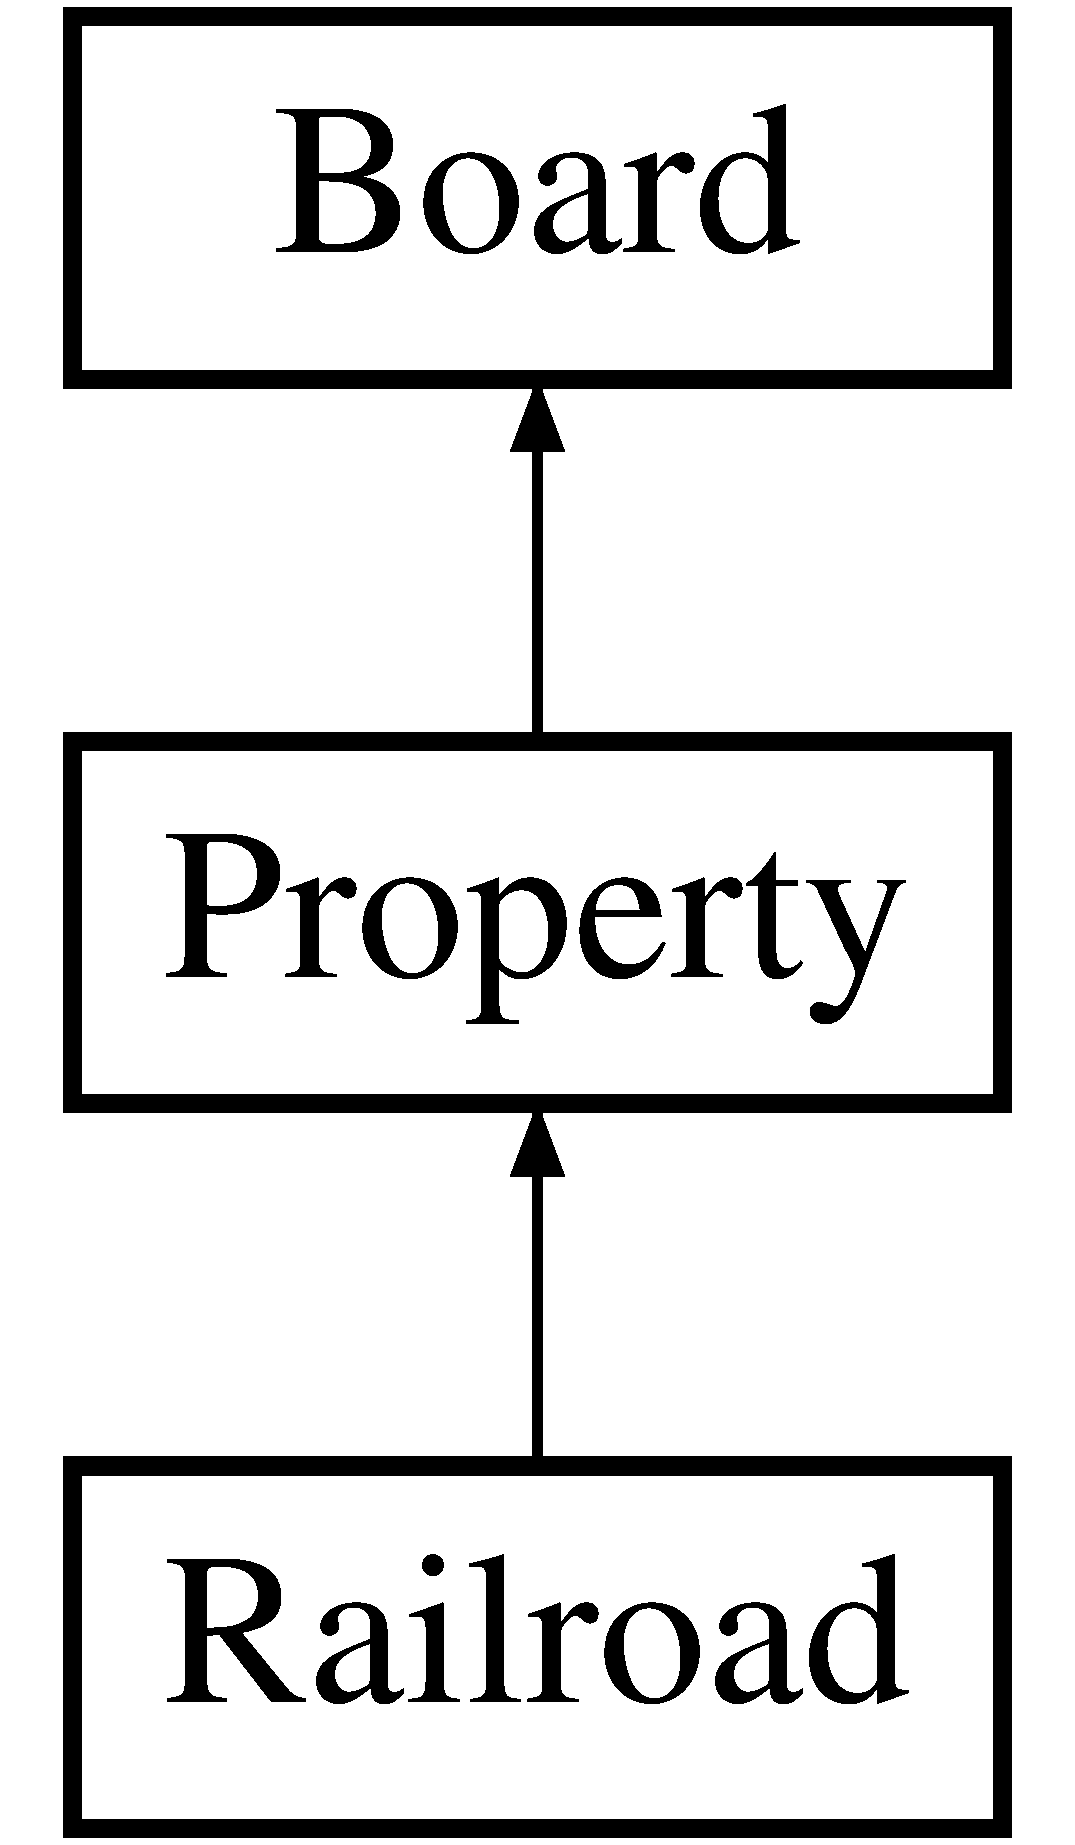
\includegraphics[height=3.000000cm]{class_board}
\end{center}
\end{figure}
\subsection*{Public Member Functions}
\begin{DoxyCompactItemize}
\item 
\mbox{\Hypertarget{class_board_af13c117dfba2e7f010f3c53dae7dab3b}\label{class_board_af13c117dfba2e7f010f3c53dae7dab3b}} 
string {\bfseries getname} () const
\item 
\mbox{\Hypertarget{class_board_acd7fadc7efd5dff9a92083ac5505ba27}\label{class_board_acd7fadc7efd5dff9a92083ac5505ba27}} 
int {\bfseries getprce} () const
\item 
\mbox{\Hypertarget{class_board_a10f8fe6e8ba0a68f130da3efc8a40ab2}\label{class_board_a10f8fe6e8ba0a68f130da3efc8a40ab2}} 
string {\bfseries getcolr} () const
\item 
\mbox{\Hypertarget{class_board_a274a3894ace6e7f0966ea1d4dd6aa459}\label{class_board_a274a3894ace6e7f0966ea1d4dd6aa459}} 
string {\bfseries col\+List} (int index)
\item 
\mbox{\Hypertarget{class_board_a55e0bccf65171a6b283d1d8fa2c4d6af}\label{class_board_a55e0bccf65171a6b283d1d8fa2c4d6af}} 
virtual void {\bfseries inform} (int, int)=0
\end{DoxyCompactItemize}
\subsection*{Protected Attributes}
\begin{DoxyCompactItemize}
\item 
\mbox{\Hypertarget{class_board_a84224bba9f78a49a9d81b6ae00404b79}\label{class_board_a84224bba9f78a49a9d81b6ae00404b79}} 
string {\bfseries name}
\item 
\mbox{\Hypertarget{class_board_aee61b2385e58ff70b14576c2269431fd}\label{class_board_aee61b2385e58ff70b14576c2269431fd}} 
int {\bfseries price}
\item 
\mbox{\Hypertarget{class_board_ad90ef830d9ea1d089deca35ecac3e4ae}\label{class_board_ad90ef830d9ea1d089deca35ecac3e4ae}} 
string {\bfseries color}
\end{DoxyCompactItemize}


The documentation for this class was generated from the following file\+:\begin{DoxyCompactItemize}
\item 
C\+:/\+Users/laurg/\+Desktop/\+C\+S\+C17\+A/\+Project/\+Project 2/\+Project2\+\_\+\+Final/Board.\+h\end{DoxyCompactItemize}

\hypertarget{class_chnc_com}{}\section{Chnc\+Com Class Reference}
\label{class_chnc_com}\index{Chnc\+Com@{Chnc\+Com}}
\subsection*{Public Member Functions}
\begin{DoxyCompactItemize}
\item 
\mbox{\Hypertarget{class_chnc_com_a805553f0f31b25257b7edd2d964a6116}\label{class_chnc_com_a805553f0f31b25257b7edd2d964a6116}} 
void {\bfseries set\+Mess} (unsigned short, short, \hyperlink{class_player}{Player} \&, \hyperlink{class_player}{Player} \&, \hyperlink{class_rules}{Rules} \&)
\item 
\mbox{\Hypertarget{class_chnc_com_ac6fb13e8c7133bbcde95263af389d11c}\label{class_chnc_com_ac6fb13e8c7133bbcde95263af389d11c}} 
string {\bfseries get\+Mess} () const
\end{DoxyCompactItemize}
\subsection*{Private Attributes}
\begin{DoxyCompactItemize}
\item 
\mbox{\Hypertarget{class_chnc_com_afaff7e4cf04aa99b258b8121ef9d883a}\label{class_chnc_com_afaff7e4cf04aa99b258b8121ef9d883a}} 
string {\bfseries message}
\end{DoxyCompactItemize}


The documentation for this class was generated from the following files\+:\begin{DoxyCompactItemize}
\item 
C\+:/\+Users/laurg/\+Desktop/\+C\+S\+C17\+A/\+Project/\+Project 2/\+Project2\+\_\+\+Final/Chnc\+Com.\+h\item 
C\+:/\+Users/laurg/\+Desktop/\+C\+S\+C17\+A/\+Project/\+Project 2/\+Project2\+\_\+\+Final/Chnc\+Com.\+cpp\end{DoxyCompactItemize}

\hypertarget{class_die}{}\section{Die Class Reference}
\label{class_die}\index{Die@{Die}}
\subsection*{Public Member Functions}
\begin{DoxyCompactItemize}
\item 
\mbox{\Hypertarget{class_die_ae4c4a9c129d6ae178f14a14b5f9725d2}\label{class_die_ae4c4a9c129d6ae178f14a14b5f9725d2}} 
void {\bfseries roll} ()
\item 
\mbox{\Hypertarget{class_die_a658a022e85993828e6a82154b048c3e2}\label{class_die_a658a022e85993828e6a82154b048c3e2}} 
int {\bfseries get\+Val} ()
\end{DoxyCompactItemize}
\subsection*{Private Attributes}
\begin{DoxyCompactItemize}
\item 
\mbox{\Hypertarget{class_die_a1d3d92c57a6d515d93162af0ca6b3e1d}\label{class_die_a1d3d92c57a6d515d93162af0ca6b3e1d}} 
int {\bfseries value}
\end{DoxyCompactItemize}


The documentation for this class was generated from the following file\+:\begin{DoxyCompactItemize}
\item 
C\+:/\+Users/laurg/\+Desktop/\+C\+S\+C17\+A/\+Project/\+Project 2/\+Project2\+\_\+\+Final/Die.\+h\end{DoxyCompactItemize}

\hypertarget{class_player}{}\section{Player Class Reference}
\label{class_player}\index{Player@{Player}}
\subsection*{Public Member Functions}
\begin{DoxyCompactItemize}
\item 
\mbox{\Hypertarget{class_player_a37fc1f766b05e107305976aa9e8d0fc4}\label{class_player_a37fc1f766b05e107305976aa9e8d0fc4}} 
void {\bfseries set\+Name} ()
\item 
\mbox{\Hypertarget{class_player_ad313d5325b68a6e80a77f02d8babd6d9}\label{class_player_ad313d5325b68a6e80a77f02d8babd6d9}} 
void {\bfseries set\+Mony} (int)
\item 
\mbox{\Hypertarget{class_player_a167fd9256e85be99d2550933a6baf5ad}\label{class_player_a167fd9256e85be99d2550933a6baf5ad}} 
void $\ast$ {\bfseries set\+Prps} ()
\item 
\mbox{\Hypertarget{class_player_af3a89c458fbed769ff76bdb398f1ea12}\label{class_player_af3a89c458fbed769ff76bdb398f1ea12}} 
void {\bfseries set\+New} (int)
\item 
\mbox{\Hypertarget{class_player_a8451a38d308061343657e96eecf0d15e}\label{class_player_a8451a38d308061343657e96eecf0d15e}} 
void {\bfseries set\+Spot} (int)
\item 
\mbox{\Hypertarget{class_player_aa8af9e54e5838a1952b0bb9686f6d8af}\label{class_player_aa8af9e54e5838a1952b0bb9686f6d8af}} 
void {\bfseries set\+N\+Hse} ()
\item 
\mbox{\Hypertarget{class_player_a9bc57b0b212853ce5b0e58bbc8a93b60}\label{class_player_a9bc57b0b212853ce5b0e58bbc8a93b60}} 
void {\bfseries set\+N\+Htl} (\hyperlink{class_property}{Property} \&)
\item 
\mbox{\Hypertarget{class_player_ad3dcd2fe41dcca95750c1c5f086479fe}\label{class_player_ad3dcd2fe41dcca95750c1c5f086479fe}} 
void {\bfseries pay\+Rent} (int)
\item 
\mbox{\Hypertarget{class_player_a4939193fc637f75bf7a11118334dae7e}\label{class_player_a4939193fc637f75bf7a11118334dae7e}} 
string {\bfseries get\+Name} () const
\item 
\mbox{\Hypertarget{class_player_a3764cbbcd74442dd129db4d7e365d5ad}\label{class_player_a3764cbbcd74442dd129db4d7e365d5ad}} 
int {\bfseries get\+Mony} () const
\item 
\mbox{\Hypertarget{class_player_a64e2d8ec271ba98488ad859a3aa03a92}\label{class_player_a64e2d8ec271ba98488ad859a3aa03a92}} 
unsigned short {\bfseries get\+N\+Prp} () const
\item 
\mbox{\Hypertarget{class_player_ab156853633779411ca1b4756645f0df4}\label{class_player_ab156853633779411ca1b4756645f0df4}} 
int {\bfseries get\+Spot} () const
\item 
\mbox{\Hypertarget{class_player_afc6a4682a635e71ca8a388f91aa20d8e}\label{class_player_afc6a4682a635e71ca8a388f91aa20d8e}} 
void $\ast$ {\bfseries get\+Prps} ()
\item 
\mbox{\Hypertarget{class_player_ac7126430a8c67db6753a75f9699db78d}\label{class_player_ac7126430a8c67db6753a75f9699db78d}} 
bool {\bfseries find\+Prp} (int)
\item 
\mbox{\Hypertarget{class_player_a4a7846d6d51a1006ecc2dba02405b340}\label{class_player_a4a7846d6d51a1006ecc2dba02405b340}} 
int {\bfseries get\+N\+Hse} () const
\item 
\mbox{\Hypertarget{class_player_ab5dc0baad7fd17bcae42387fc1fdb764}\label{class_player_ab5dc0baad7fd17bcae42387fc1fdb764}} 
int {\bfseries get\+N\+Htl} () const
\end{DoxyCompactItemize}
\subsection*{Protected Attributes}
\begin{DoxyCompactItemize}
\item 
\mbox{\Hypertarget{class_player_a9545beef70350d5c3b3a5719a890dd2f}\label{class_player_a9545beef70350d5c3b3a5719a890dd2f}} 
int {\bfseries money}
\end{DoxyCompactItemize}
\subsection*{Private Attributes}
\begin{DoxyCompactItemize}
\item 
\mbox{\Hypertarget{class_player_acf0355128a99ee20ad9931b760fb2de1}\label{class_player_acf0355128a99ee20ad9931b760fb2de1}} 
string {\bfseries name}
\item 
\mbox{\Hypertarget{class_player_ae2bb900a8eaa9f44058edce4fd116e0d}\label{class_player_ae2bb900a8eaa9f44058edce4fd116e0d}} 
unsigned short {\bfseries n\+Props}
\item 
\mbox{\Hypertarget{class_player_ae8e6a6cc0177624e8ed30b8f95f049c0}\label{class_player_ae8e6a6cc0177624e8ed30b8f95f049c0}} 
int $\ast$ {\bfseries proprty}
\item 
\mbox{\Hypertarget{class_player_a572b8db7cfdd88a9af932a1f7a610641}\label{class_player_a572b8db7cfdd88a9af932a1f7a610641}} 
int {\bfseries spot}
\item 
\mbox{\Hypertarget{class_player_ab90c8c07e91ee36012185229c5abc3d7}\label{class_player_ab90c8c07e91ee36012185229c5abc3d7}} 
int {\bfseries out\+Jail}
\item 
\mbox{\Hypertarget{class_player_ab151fc3b7160af7b89ca356ac5107d4d}\label{class_player_ab151fc3b7160af7b89ca356ac5107d4d}} 
int {\bfseries n\+Houses}
\item 
\mbox{\Hypertarget{class_player_aa0ac76798f3a75d5163b9fb887e4c7a3}\label{class_player_aa0ac76798f3a75d5163b9fb887e4c7a3}} 
int {\bfseries n\+Hotels}
\end{DoxyCompactItemize}
\subsection*{Friends}
\begin{DoxyCompactItemize}
\item 
\mbox{\Hypertarget{class_player_ae6db878679688c4d56ae2e97c86c6725}\label{class_player_ae6db878679688c4d56ae2e97c86c6725}} 
void {\bfseries Chnc\+Com\+::set\+Mess} (unsigned short, short, \hyperlink{class_player}{Player} \&, \hyperlink{class_player}{Player} \&, \hyperlink{class_rules}{Rules} \&)
\item 
\mbox{\Hypertarget{class_player_aa34775e5581bc3473f4da48e27e0aff6}\label{class_player_aa34775e5581bc3473f4da48e27e0aff6}} 
void {\bfseries Rules\+::\+Go2\+Jail} (\hyperlink{class_player}{Player} \&)
\item 
\mbox{\Hypertarget{class_player_ad64d486925f00c04d73ee000fd856b37}\label{class_player_ad64d486925f00c04d73ee000fd856b37}} 
void {\bfseries Rules\+::c\+Go\+Jail} (\hyperlink{class_player}{Player} \&)
\item 
\mbox{\Hypertarget{class_player_a45bcb466a41cb86f9ee8ebfba7a1b1d4}\label{class_player_a45bcb466a41cb86f9ee8ebfba7a1b1d4}} 
void {\bfseries Rules\+::restart} (int, \hyperlink{class_player}{Player} \&)
\item 
\mbox{\Hypertarget{class_player_a17ae887e285346988c33e45f9b9d9389}\label{class_player_a17ae887e285346988c33e45f9b9d9389}} 
ostream \& {\bfseries operator$<$$<$} (ostream \&, const \hyperlink{class_player}{Player} \&)
\end{DoxyCompactItemize}


The documentation for this class was generated from the following files\+:\begin{DoxyCompactItemize}
\item 
C\+:/\+Users/laurg/\+Desktop/\+C\+S\+C17\+A/\+Project/\+Project 2/\+Project2\+\_\+\+Final/Player.\+h\item 
C\+:/\+Users/laurg/\+Desktop/\+C\+S\+C17\+A/\+Project/\+Project 2/\+Project2\+\_\+\+Final/Player.\+cpp\end{DoxyCompactItemize}

\hypertarget{class_property}{}\section{Property Class Reference}
\label{class_property}\index{Property@{Property}}
Inheritance diagram for Property\+:\begin{figure}[H]
\begin{center}
\leavevmode
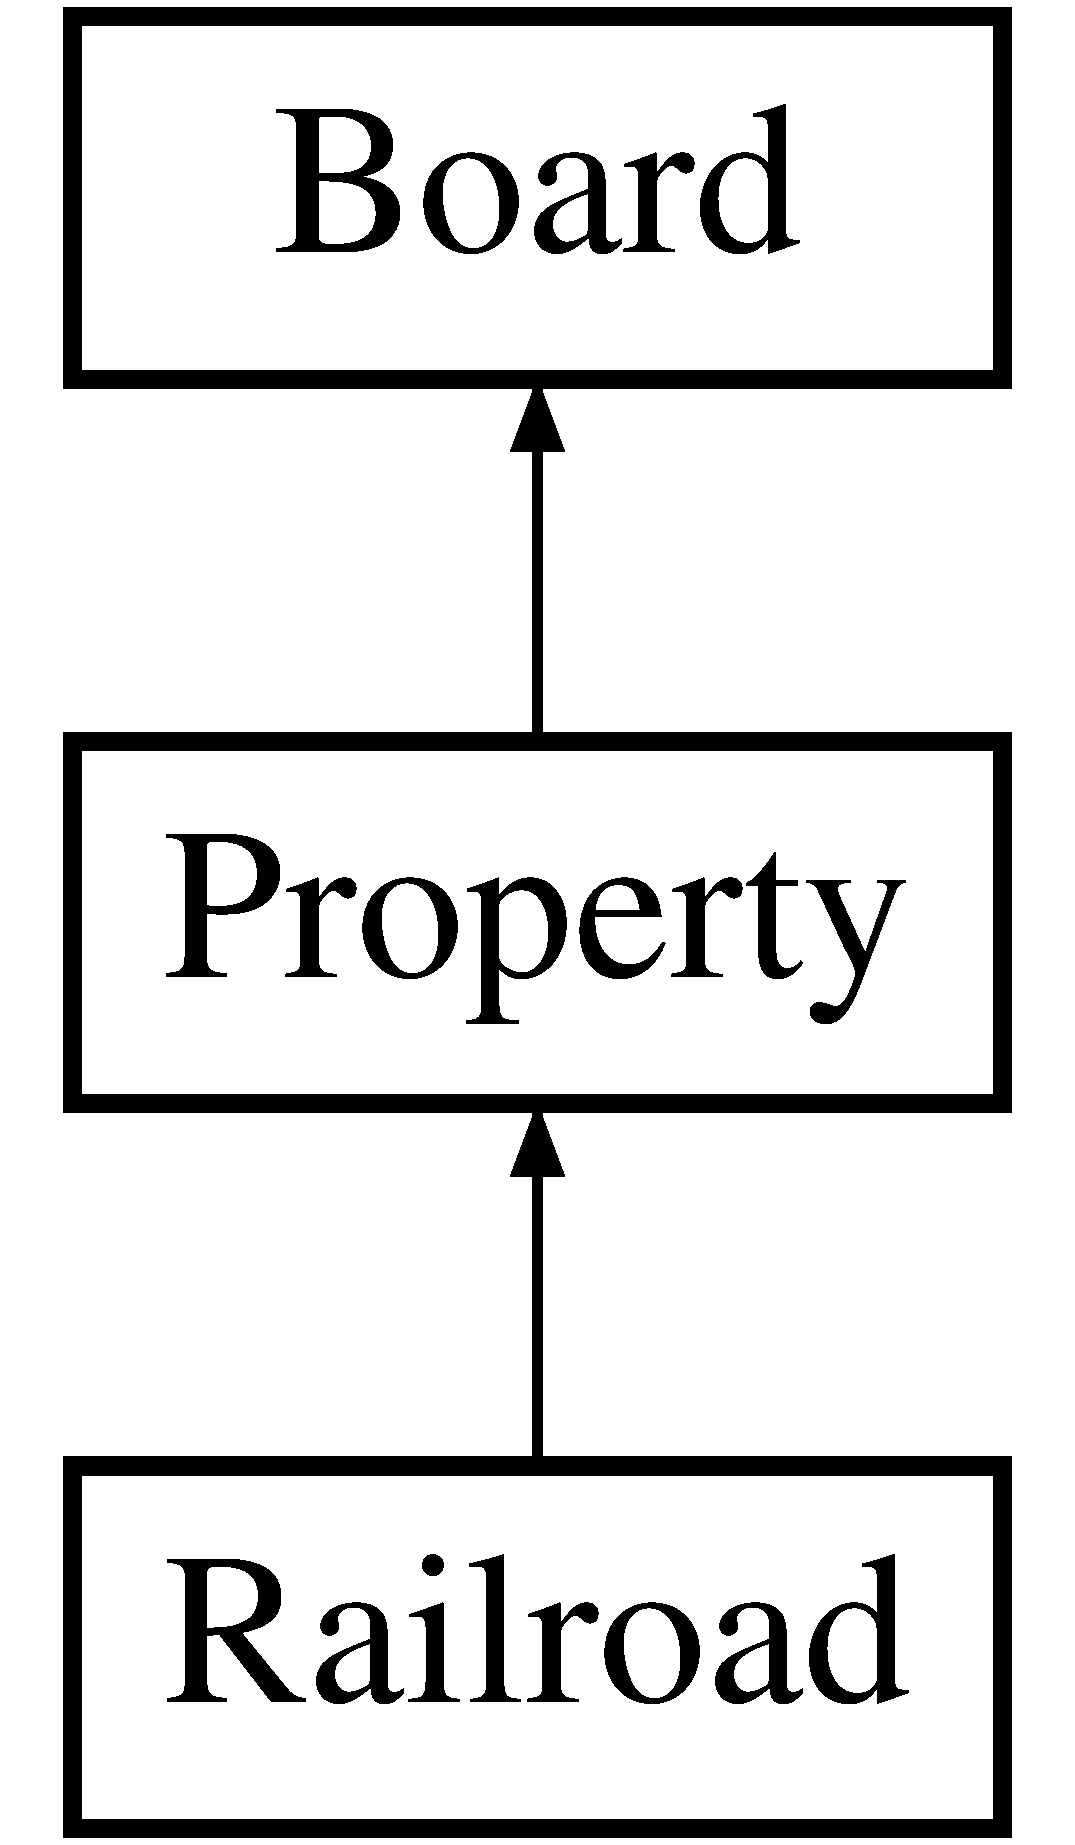
\includegraphics[height=3.000000cm]{class_property}
\end{center}
\end{figure}
\subsection*{Public Member Functions}
\begin{DoxyCompactItemize}
\item 
\mbox{\Hypertarget{class_property_a505911a3207cee21c2e656ab9ee794a7}\label{class_property_a505911a3207cee21c2e656ab9ee794a7}} 
int {\bfseries getrent} () const
\item 
\mbox{\Hypertarget{class_property_a0f2941a1cfa79baba73ad58f7fb77978}\label{class_property_a0f2941a1cfa79baba73ad58f7fb77978}} 
int {\bfseries get\+HseC} () const
\item 
\mbox{\Hypertarget{class_property_acd727a8ccda5e79aa865205dc4ad5aa3}\label{class_property_acd727a8ccda5e79aa865205dc4ad5aa3}} 
int {\bfseries get\+HtlC} () const
\item 
\mbox{\Hypertarget{class_property_ad0e3b17c171e2bbb79ea923e1556ea40}\label{class_property_ad0e3b17c171e2bbb79ea923e1556ea40}} 
int {\bfseries setc\+Max} (string)
\item 
\mbox{\Hypertarget{class_property_a824ac426fc7afbf163522586aa7d844e}\label{class_property_a824ac426fc7afbf163522586aa7d844e}} 
{\footnotesize template$<$class T1 , class T2 $>$ }\\void {\bfseries util\+Rnt} (T1 \&number, T2 \&util)
\item 
\mbox{\Hypertarget{class_property_ab3f16b101b063cd7f1b7aa059595a714}\label{class_property_ab3f16b101b063cd7f1b7aa059595a714}} 
virtual string {\bfseries get\+Pos} (int named) const
\item 
\mbox{\Hypertarget{class_property_af8ee451681c0cfb0d90c417772776e5c}\label{class_property_af8ee451681c0cfb0d90c417772776e5c}} 
virtual void {\bfseries inform} (int, int)
\end{DoxyCompactItemize}
\subsection*{Protected Attributes}
\begin{DoxyCompactItemize}
\item 
\mbox{\Hypertarget{class_property_a04e947c064fb7d02ac757335e5d7e583}\label{class_property_a04e947c064fb7d02ac757335e5d7e583}} 
int {\bfseries rent}
\end{DoxyCompactItemize}
\subsection*{Private Attributes}
\begin{DoxyCompactItemize}
\item 
\mbox{\Hypertarget{class_property_ad09061ba30d1ea3df659f1555b998fc3}\label{class_property_ad09061ba30d1ea3df659f1555b998fc3}} 
int {\bfseries hse\+Cost}
\item 
\mbox{\Hypertarget{class_property_a87c4d4ebc92499b0337272e4aedfed53}\label{class_property_a87c4d4ebc92499b0337272e4aedfed53}} 
int {\bfseries htl\+Cost}
\item 
\mbox{\Hypertarget{class_property_af26458d798fdd15493edf5b72ff7f18f}\label{class_property_af26458d798fdd15493edf5b72ff7f18f}} 
int {\bfseries max\+Colr}
\end{DoxyCompactItemize}


The documentation for this class was generated from the following files\+:\begin{DoxyCompactItemize}
\item 
C\+:/\+Users/laurg/\+Desktop/\+C\+S\+C17\+A/\+Project/\+Project 2/\+Project2\+\_\+\+Final/Property.\+h\item 
C\+:/\+Users/laurg/\+Desktop/\+C\+S\+C17\+A/\+Project/\+Project 2/\+Project2\+\_\+\+Final/Property.\+cpp\end{DoxyCompactItemize}

\hypertarget{class_railroad}{}\section{Railroad Class Reference}
\label{class_railroad}\index{Railroad@{Railroad}}
Inheritance diagram for Railroad\+:\begin{figure}[H]
\begin{center}
\leavevmode
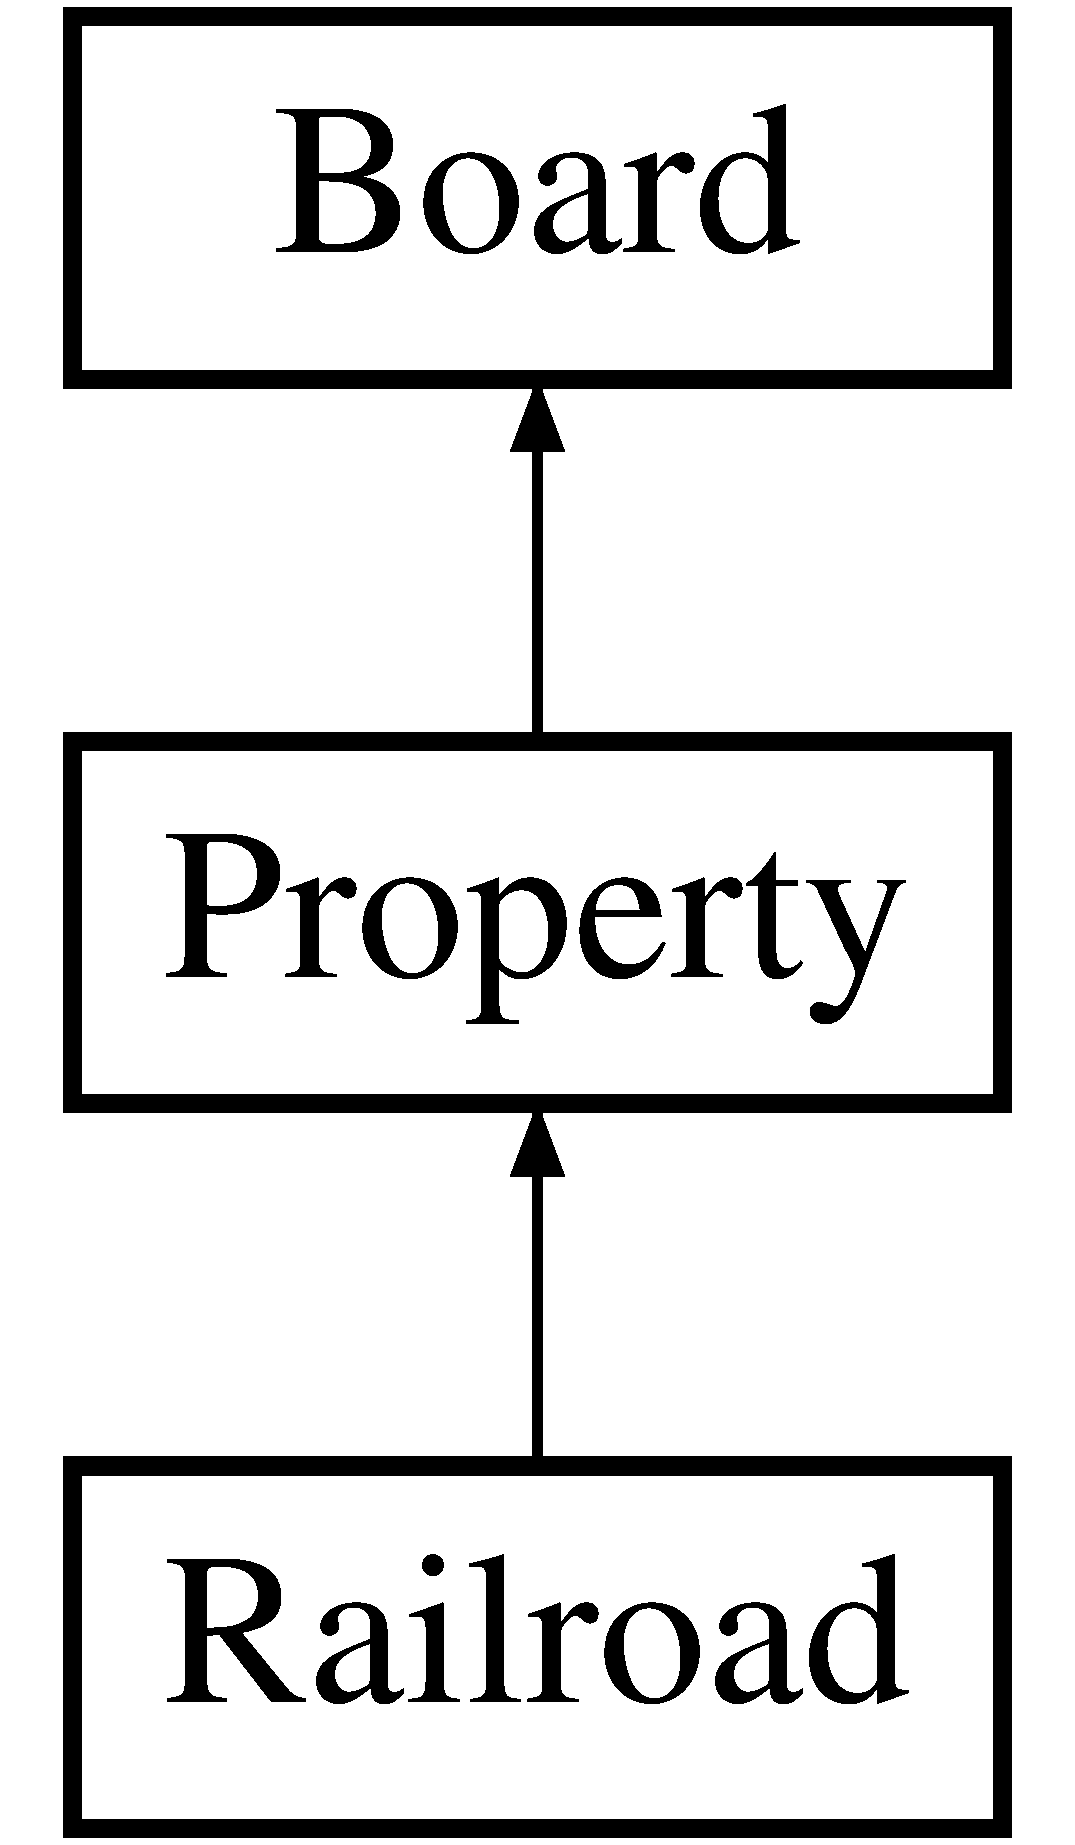
\includegraphics[height=3.000000cm]{class_railroad}
\end{center}
\end{figure}
\subsection*{Public Member Functions}
\begin{DoxyCompactItemize}
\item 
\mbox{\Hypertarget{class_railroad_a484c95e6479fec5cc20e317554c8d1b7}\label{class_railroad_a484c95e6479fec5cc20e317554c8d1b7}} 
int {\bfseries setrent} (\hyperlink{class_player}{Player} \&player, int current)
\item 
\mbox{\Hypertarget{class_railroad_a7c0c4afa3aaaf47af9120ab23512983e}\label{class_railroad_a7c0c4afa3aaaf47af9120ab23512983e}} 
virtual string {\bfseries get\+Pos} (int named) const
\end{DoxyCompactItemize}
\subsection*{Additional Inherited Members}


The documentation for this class was generated from the following file\+:\begin{DoxyCompactItemize}
\item 
C\+:/\+Users/laurg/\+Desktop/\+C\+S\+C17\+A/\+Project/\+Project 2/\+Project2\+\_\+\+Final/Railroad.\+h\end{DoxyCompactItemize}

\hypertarget{class_rules}{}\section{Rules Class Reference}
\label{class_rules}\index{Rules@{Rules}}
\subsection*{Public Member Functions}
\begin{DoxyCompactItemize}
\item 
\mbox{\Hypertarget{class_rules_a7f5e6a12c1b392a9e56d58877c2a46c6}\label{class_rules_a7f5e6a12c1b392a9e56d58877c2a46c6}} 
void {\bfseries Go2\+Jail} (\hyperlink{class_player}{Player} \&)
\item 
\mbox{\Hypertarget{class_rules_a567307b732f394e528383293d91fbde5}\label{class_rules_a567307b732f394e528383293d91fbde5}} 
void {\bfseries c\+Go\+Jail} (\hyperlink{class_player}{Player} \&)
\item 
\mbox{\Hypertarget{class_rules_a6377ce4bb12df15cdf914403c3031451}\label{class_rules_a6377ce4bb12df15cdf914403c3031451}} 
void {\bfseries restart} (int, \hyperlink{class_player}{Player} \&)
\item 
\mbox{\Hypertarget{class_rules_a8bfdb512617cfa624152232228da73c6}\label{class_rules_a8bfdb512617cfa624152232228da73c6}} 
void {\bfseries indxset} (short \&)
\item 
\mbox{\Hypertarget{class_rules_a5641a3d79e65d103fa9263e4a10f9566}\label{class_rules_a5641a3d79e65d103fa9263e4a10f9566}} 
bool {\bfseries game\+End} (\hyperlink{class_player}{Player} \&)
\end{DoxyCompactItemize}
\subsection*{Private Attributes}
\begin{DoxyCompactItemize}
\item 
\mbox{\Hypertarget{class_rules_a3ee34eda1062303e7c36c71a804b9ded}\label{class_rules_a3ee34eda1062303e7c36c71a804b9ded}} 
int {\bfseries leftovr}
\item 
\mbox{\Hypertarget{class_rules_ad9052569712c9c1b9c25177e58a5e752}\label{class_rules_ad9052569712c9c1b9c25177e58a5e752}} 
int {\bfseries extra}
\end{DoxyCompactItemize}
\subsection*{Friends}
\begin{DoxyCompactItemize}
\item 
\mbox{\Hypertarget{class_rules_ae6db878679688c4d56ae2e97c86c6725}\label{class_rules_ae6db878679688c4d56ae2e97c86c6725}} 
void {\bfseries Chnc\+Com\+::set\+Mess} (unsigned short, short, \hyperlink{class_player}{Player} \&, \hyperlink{class_player}{Player} \&, \hyperlink{class_rules}{Rules} \&)
\end{DoxyCompactItemize}


The documentation for this class was generated from the following files\+:\begin{DoxyCompactItemize}
\item 
C\+:/\+Users/laurg/\+Desktop/\+C\+S\+C17\+A/\+Project/\+Project 2/\+Project2\+\_\+\+Final/Rules.\+h\item 
C\+:/\+Users/laurg/\+Desktop/\+C\+S\+C17\+A/\+Project/\+Project 2/\+Project2\+\_\+\+Final/Rules.\+cpp\end{DoxyCompactItemize}

%--- End generated contents ---

% Index
\backmatter
\newpage
\phantomsection
\clearemptydoublepage
\addcontentsline{toc}{chapter}{Index}
\printindex

\end{document}
